\documentclass[12pt, twoside]{article}
\usepackage[letterpaper, margin=1in, headsep=0.5in]{geometry}
\usepackage[english]{babel}
\usepackage[utf8]{inputenc}
\usepackage{amsmath}
\usepackage{amsfonts}
\usepackage{amssymb}
\usepackage{tikz}
%\usetikzlibrary{quotes, angles}

\usepackage{graphicx}
\usepackage{enumitem}
\usepackage{multicol}

\usepackage{fancyhdr}
\pagestyle{fancy}
\fancyhf{}
\renewcommand{\headrulewidth}{0pt} % disable the underline of the header

\fancyhead[LE]{\thepage}
\fancyhead[RO]{\thepage \\ Name: \hspace{4cm} \,\\}
\fancyhead[LO]{BECA / Dr. Huson / Geometry\\* Unit 7: Similarity\\* 13 January 2020}

\begin{document}
\subsubsection*{7.8 Homework: Right triangle ratios, constructions}
  \begin{enumerate}

  \begin{multicols}{2}[\item In $\triangle ABC$ shown below, $\angle ACB$ is a right angle, $E$ is a point on $\overline{AC}$, and $\overline{ED}$ is drawn perpendicular to hypontenuse $\overline{AB}$. Given $\triangle ABC \sim \triangle AED$.]
    \begin{enumerate}[itemsep=0.7cm]
      \item Justify $\angle BAC \cong \angle EAD$.
      \item $\angle B \rightarrow$ \quad \rule{2cm}{0.15mm} 
      \item $\overline{AC} \rightarrow$ \quad \rule{2cm}{0.15mm}
      \item $DE = k \times $ \ \rule{2cm}{0.15mm}
      \end{enumerate}
      \begin{center}
        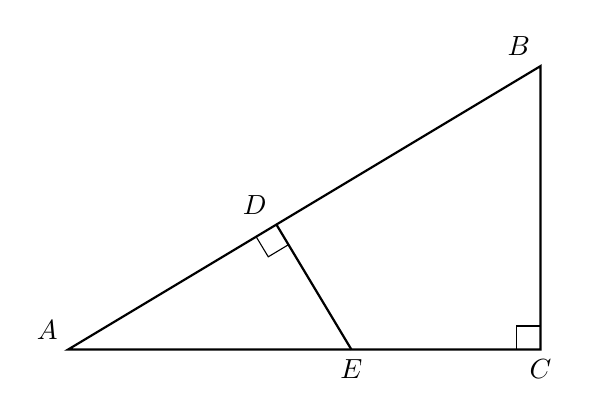
\begin{tikzpicture}[scale=0.6]
          \draw [-, thick] (0,0) node[above left]{$A$}--
          (10,0) node[below]{$C$}--
          (10,6) node[above left]{$B$}--cycle;
          \draw [thick] (6,0)--(4.41,2.65);
          \node at (6,0) [below]{$E$};
          \node at (4.41,2.65) [above left]{$D$};
          \draw (10,0) ++(-0.5,0)--++(0,0.5)--++(0.5,0);
          \draw (4.41,2.65) ++(-59:0.5)--++(-149:0.5)--++(121:0.5);
          %\node at (4, 0) [below]{$12$};
          %\node at (3,2) [above]{$9$};
          %\node at (9, 3) [right]{$10$};
          %\node at (5.5, 1.6) [right]{$6$}; \vspace{1cm}
        \end{tikzpicture}
      \end{center} 
    \end{multicols}
      %\vspace{1cm}

  \begin{multicols}{2}[\item In $\triangle ABC$ shown below, $\angle ACB$ is a right angle, and $\overline{CD} \perp \overline{AB}$.]
        \begin{enumerate}[itemsep=0.5cm]
          \item Name three similar triangles (ordering the letters in proper correspondence). \vspace{1cm}
          \item T \quad F \quad $\displaystyle \frac{BD}{BC}= \frac{CD}{AC}$
          \item T \quad F \quad $\displaystyle \frac{AB}{AC}= \frac{BC}{AD}$
          \item T \quad F \quad $AD \times BD = CD \times CD$
          \columnbreak
          \end{enumerate}
          \begin{center}
            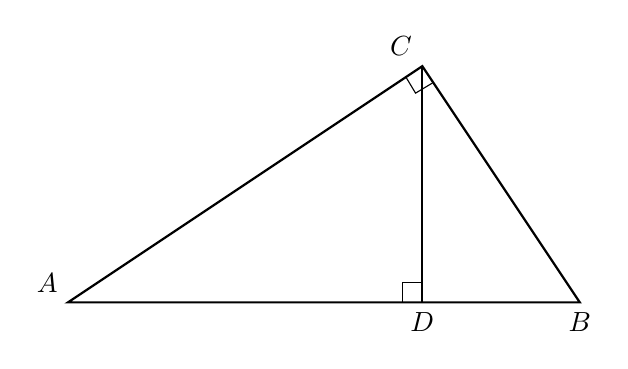
\begin{tikzpicture}[scale=0.5]
              \draw [-, thick] (-9,0) node[above left]{$A$}--
              (4,0) node[below]{$B$}--
              (0,6) node[above left]{$C$}--cycle;
              \draw [thick] (0,6)--(0,0)node[below]{$D$};
              \draw (0,0) ++(-0.5,0)--++(0,0.5)--++(0.5,0);
              \draw (0,6) ++(-59:0.5)--++(-149:0.5)--++(121:0.5);
              %\node at (4, 0) [below]{$12$};
              %\node at (3,2) [above]{$9$};
              %\node at (9, 3) [right]{$10$};
              %\node at (5.5, 1.6) [right]{$6$}; \vspace{1cm}
            \end{tikzpicture}
          \end{center} 
        \end{multicols}
          %\vspace{1cm}

  \item In the diagram below, the chords $\overline{AE}$ and $\overline{BD}$ intersect at $C$.
    \begin{multicols}{2}
      \begin{enumerate}[itemsep=0.5cm]
        \item What angle corresponds with $\angle E$?
        \item T \quad F \quad $\displaystyle \frac{CE}{BC}= \frac{CD}{AC}$
        \item T \quad F \quad $AC \times CE = BC \times CD$    
      \end{enumerate}
      \columnbreak
      \begin{flushright}
      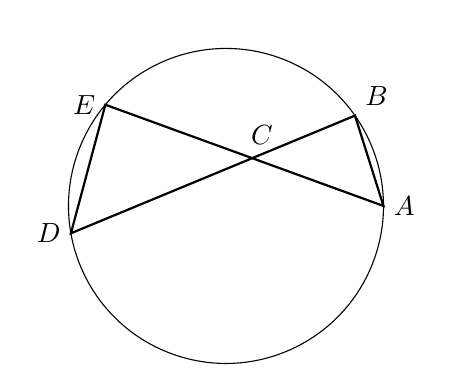
\begin{tikzpicture}[rotate=-20, scale=.4]
        \draw (0,0) circle[radius=5];
        \draw [thick]
        (20:5) node[right] {$A$}--
        (160:5) node[left] {$E$}--
        (210:5) node[left] {$D$}--
        (55:5) node[above right] {$B$}--cycle;
        \draw (75:2) node[above] {$C$};
      \end{tikzpicture}
    \end{flushright}
  \end{multicols}

\newpage
  \item Complete the construction of a perpendicular bisector of $\overline{AB}$. Label the midpoint $M$. Show all construction marks, but make no extra lines. \vspace{2cm}
    \begin{center}
    \begin{tikzpicture}
      \draw [-, thick] (0,0)--(4,5);
      \draw [fill] (0,0) circle [radius=0.05] node[below right]{$A$};
      \draw [fill] (4,5) circle [radius=0.05] node[above left]{$B$};
    \end{tikzpicture}
    \end{center} \vspace{4cm}

  \item Accurately draw a square that is 5 centimeters on each side.

\newpage
  \item Complete the construction of an equilateral triangle with one side as $\overline{XY}$. Show all construction marks, but make no extra lines. \vspace{3cm}
  \begin{center}
  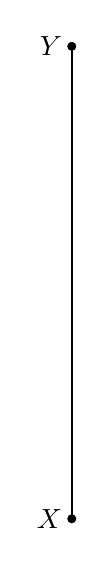
\begin{tikzpicture}
    \draw [-, thick] (0,0)--(0,6);
    \draw [fill] (0,0) circle [radius=0.05] node[left]{$X$};
    \draw [fill] (0,6) circle [radius=0.05] node[left]{$Y$};
  \end{tikzpicture}
  \end{center} \vspace{3cm}
  \begin{enumerate}
    \item Identify two circles in the construction. For each, name the center of the circle and the radius.  \vspace{3cm}
    \item Assuming that the third vertex of the triangle is point $Z$, explain why the distance from $X$ to $Z$ is the same as the distance from $X$ to $Y$.
  \end{enumerate}

\newpage
  \item Complete the construction of a line perpendicular to line $l$ through the point $P$. Show all construction marks, but make no extra lines. \vspace{3cm}
  \begin{center}
  \begin{tikzpicture}
    \draw [<->, thick] (-5,0)--(7,0)node[below]{$l$}--(8,0);
    \draw [fill] (3,3) circle [radius=0.05] node[above left]{$P$};
  \end{tikzpicture}
  \end{center} \vspace{7cm}

  \item The perimeter of a square is 52 cm. Find the area of the square.


\end{enumerate}
\end{document}